\chapter{Implementation} \label{cha:impl}

This section will focus on the implementation of the zero core \gls{ide}. In
section \ref{sec:stack}, we will mention technologies used, and why they were
chosen. In section \ref{sec:mod1} and \ref{sec:mod2}, we will discuss the
different iterations the application architecture had, and why they were subpar,
compared to section \ref{sec:mod3}, which is the implementation of the zero core
\gls{ide}. Section \ref{sec:testing} will explain the necessity of testing when
using such a modular design, and explore the ease of which functionality can be
tested.

\section{Tech Stack} \label{sec:stack}

A module can extend an application at either compile time, or during runtime.
This could be achieved by using an interpreted language like JavaScript or
Python. The issue with using a dynamically typed language like Python or
JavaScript, is that it enhances the risk for runtime issues occurring, and when
dealing with scenarios like writing to files, or running long processes like
compiling a program, it is important to avoid such issues. So using a typesafe
language, that can \textit{transform} runtime errors into compile time errors,
is preferred. Furthermore, being able to support runtime modules, in a language
agnostic manner, necessarily means that the core \gls{ide} needs good
\gls{abi} support, and therefore should be implemented in a low level language.
But what does \textit{low level} language mean? And what is an \gls{abi}?

\subsection{Low level languages}

Programming languages has changed over time. In the beginning, a program was a
series of ones and zeros, representing instructions a computer should do. Since
then, we have moved several abstraction layers above what is commonly referred
as \textit{bare metal} programming. From writing in hexadecimal instead of
binary, to machine instructions, to more generic programming language, like C.
What was different with C, compared to writing direct machine instructions, was
that an external program, a compiler, could translate C code to machine
instructions specific to the computers' \gls{cpu} architecture, this meant a
single program, written in C, could be compiled to many different computers. So,
at the time C came out, it was considered a \textit{high level} programming
language, because the language a developer was writing in, had a higher level of
abstraction. Today this notion of \textit{low} and \textit{high} level languages
has changed. A \textit{low level} language is close to how a \gls{cpu}
\textit{thinks}, which has traditionally meant that C is a low level programming
language, but some authors \cite{cNotLowLevel} argue that this is no longer the
case. In any case, we will use \textit{low level} to mean a programming
languages like C, where direct memory manipulations is a feature of the
language.

\subsection{Application Binary Interface (ABI)}

An \gls{abi} is an low-level interface, a kind of \gls{api},
between two programs. Such as C program and its dynamic library dependencies.
The \gls{abi} defines how data is laid out in memory, how functions are
invoked, and other machine level details. Both the C program and the dynamic
libraries must agree on the \gls{abi}, otherwise misinterpreted data or invalid
function calls could lead to \gls{ub}.

\paragraph{Undefined behavior} In programming \gls{ub} occurs when a program
violates the language specification in a manner that is not defined by the
specification. This can be the results of \gls{abi} mismatch, like if the
layout of a struct in memory differs between the parties, in a manner which
leads to breaking of type safety, or direct violations of the language rules,
like null pointer dereference. \gls{ub} is dangerous because the compiler might
optimize the binary unpredictably or the program may behave arbitrary. It is
also a vector of attack for hackers.

\paragraph{Why not C?} C has good parts, like the C-\gls{abi}, which most
languages have bindings too. Using C would mean allowing those languages to
interface with our project, meaning, one step closer to a language agnostic
module architecture. But C has issues, like being the number one cause in
security issues. (This is just because so much of our infrastructure is written
in C, but y'know.) These security issues are mostly caused by memory management.
Would be cool if the C compiler could notify a developer if they were developing
something that could cause an issue in the future. Enter, Rust.

\subsection{Rust}

Rust is a general purpose programming language, designed for, amongst other
things, type safety, memory safety, and concurrency. When programming in Rust,
the bugs common in other languages, like null pointers, buffer overflow and data
races are detected at compile time. Most of these are features of Rusts
ownership rules. These rules, enforced by the compiler, ensure that values are
safely dropped, (freed), this ensures that all variables referenced in Rust have
a value, and can be safely evaluated. It works by simply dropping values when
they are out of scope. The example in listing \ref{lst:ownership}, the
\textbf{name} variable is declared, and used as an argument in the
\textbf{greeting} function. We cannot call the function again with
\textbf{name}, since at the end of \textbf{greeting}, before it returns,
\textbf{name} is dropped, since once we called \textbf{greeting}, the
\textbf{main} method no longer \textit{owned} \textbf{name}, as the ownership
was transferred to \textbf{greeting}. We could \textit{fix} this by changing the
argument type from \textit{name: String}, to \textit{name: \&String}, (commonly
written as \textit{name: \&str}), and adding the borrow symbol to the argument in
the method invocation, as shown in listing \ref{lst:ownership-ref}.

\begin{center}
  \lstinputlisting
    [ language=Rust
    , caption={Ownership example (Rust)}
    , label=lst:ownership
    ]{./code/rust-ownership.rs}
\end{center}

\begin{center}
  \lstinputlisting
    [ language=Rust
    , caption={Ownership example with reference (Rust)}
    , label=lst:ownership-ref
    ]{./code/rust-ownership-ref.rs}
\end{center}

This same principle ensure the other mentioned features of the language,
including performance, as with the borrow checker, there is no need for a
garbage collector. Another Rust feature are so-called \textit{macros}. A macro
is some code that is evaluated and executed at compile time, that may change
the source code. An example of this, can be seen in listing \ref{lst:ownership}.
The \textbf{println!} is a macro invocation. \textbf{println!} is used so that
the developer doesn't have to format the expressions being used, this is handled
by the macro. This is helpful because redundant work can be automated.

Furthermore, Rust has good cross-platform support, ensuring
we can write OS-agnostic code, and compile it to specific targets, without much
hassle. Since Rust is low-level, it has good bindings to C, ensuring
compatibility with future models, made in other languages, by use of the Rust
\gls{abi}.

\subsubsection{Rust Application Binary Interface}

Rust's \gls{abi} is not stable! Because it is not supported by their semantic
versioning. This means even a bug fix in the compiler, could break the
\gls{abi}. So if an application, written in Rust, is compiled in version 1.8.0,
if this application relies on a Rust library that is compiled in version 1.8.0,
everything is okay. But if the application is later recompiled with a compiler
in version 1.8.1, then \textit{undefined} behavior could occur. One of the ways
undefined behavior was avoided, was using the \textit{abi\_stable}-crate, which
enables \textit{safe} loading of external libraries, meaning modules. This is
only an issue for runtime modules, which means they need to be handled
differently than compile time modules.

If the types in the core application change, either by expansion or renaming or
such, the crate would crash the application during startup, because the existing
module would have a different expectation of what types existed, which again,
could lead to undefined behavior. But, this due to the implementation of a
runtime module using the \textit{abi\_stable}-crate, as one could design a
module to be expanded in the future, but due to the stability of the \gls{api},
this was deemed unnecessary.

\subsection{Tauri}

Tauri is a framework for Rust, which enables us to create a cross-platform
application. Any frontend framework that compiles to \gls{html}, JavaScript and
\gls{css} can be used as the \gls{gui}. Such a \gls{gui} is commonly referred to
as a \textit{web view}. This framework also adds support for invoking Rust
methods in the frontend framework, and vice-versa. This allows for support of
JavaScript modules, without much fuzz. Tauri archives with \gls{ipc}, which
allows for isolated processes to communicate securely. For JavaScript to Rust,
this is achieved with something called \textit{Commands}, which acts as an
abstraction on top of the \gls{ipc}, which turns the invocation to a
frontend-backend architecture.

\subsubsection{TypeScript}

Any frontend framework that compiles to \gls{html}, JavaScript and \gls{css} can
be used with Tauri, so TypeScript was chosen. TypeScript offers a lot of
features over JavaScript, amongst them being able to \textit{type} functions,
ensuring null/undefined-safety. Furthermore, by using crates like
\textit{ts-rs}, Rust types can be annotated with attribute macros, which create
a one-to-one mapping between the Rust type, and the serialized JSON object, to
be used in TypeScript, allowing for even more type safety, and ensuring that the
types used in the \gls{ide} only have to be defined one place.

Allowing for any JavaScript library to be used, enabled a low development time
of \gls{ui} components, since this is something that a lot of \gls{ui} and user
experience designers have looked into. So existing code for this already exists
and can be used. \gls{npm}, for example, is a package registry for JavaScript.
It contains around \textit{34 million} libraries, all of which are usable in
this architecture. If the functionality that these libraries are useful for the
application, is another question. This functionality allows for quick
development time for modules, which means features that are standard in
\gls{ide} can be quickly and easily added.

\subsection{Security}

This framework gives a lot of security which is needed in an
application which runs third party code.
\todo{Look into isolation pattern from Tauri}

\subsubsection{Module Validation}

Running third-party-code can dangerous. If this code is not validated or does
not come from a trusted source, it could be an attack vector. Luckily, Tauri does
some of this work for us, allowing us to analyze all module to core
communication, but even if we have validated that a module is wanted, there is
still the remaining use that has been the reason for 100\% of all CVE's, human
error.

The Rust compiler can ensure that the Rust modules are valid during compile
time, for runtime this is a bit trickier. But for JavaScript modules, which the
\gls{ide} supports out-of-the-box, this is a bigger issue. This lead to the
development of two systems. \gls{rsms} and \gls{jsms}.

It was necessary to distinguish the different module systems, due to the way
they would be loaded and invoked by the core application. Since the core is
written in Rust, the \gls{rsms} doesn't have to do any validation or
translation when communicating with compile time modules. With runtime modules
this also ended up being trivial, but will be discussed more in depth later.

In the \gls{jsms}, managing of modules can lead to exceptions being thrown.
Since third party code is being run, nothing can be trusted. All module
invocations and outputs needs to be sanitized before it can be used in the core
application. This is achieved by wrapping all invocations in a
\textit{try-catch}, and using the \textit{io-fp} library to decode types during
runtime. This enables us to safely invoke modules, as we can translate all
computations into a product type, where it is either a success, giving us the
wanted computation from the module, or an error. But even with types, we cannot
verify functions. Since during runtime, we are in the JavaScript environment,
we can only validate if something is a function, using the
\lstinline[language=JavaScript]{typeof} operator. It is possible to do
\textit{some} verification on functions in JavaScript, but this is only a) Is it
a function, and b) does it have the correct amount of arguments. In this case,
one. Nothing about the typing of the function can be ascertained at runtime,
without explicitly invoking the function.

\section{Module V.1} \label{sec:mod1}

We did not attempt at first, to create a zero core application; this was a
\textit{natural} conclusion to the existing problem. The first attempt was a
simple generic \gls{ide}, in which the module architecture was a concern from
day one of development. The general plan was this:

\begin{enumerate}
  \item Create an \gls{ide}
  \item Extend the \gls{ide}, to allow for a module architecture
  \item Modules call the application using some DSL
\end{enumerate}

Since any JavaScript frontend framework could be used, React was chosen, one of
the reason for this choice was due to its popularity, which again, would speed
up the development time of the application, but also due to the way React
renders the \gls{html}. Between two different re-renders of the application,
React can check the difference between the \gls{vdom}, which is React's
representation of the \gls{dom}. It then only changes what is needed in the
\gls{dom}, instead of re-creating the entire \gls{dom}, which makes the render
time quick.

This was the more straight forward way to work, because as we could model it of
existing \gls{ide}s, like \textit{Visual Studio Code} or \textit{Eclipse}.
Another advantage is that when implementing the application, one necessarily
gets a better understand of how eventual modules should extend the application.

This approach did unfortunately not lead to a truly modular application. Similar
issues to existing \gls{ide}s, how does one allow for \textit{everything}?
Furthermore, anything created this way, would be subpar to existing software,
which would lead to the next maintainer having to fix the core application. This
in turn, would add a lot of complexity, which the maintainers would have to deal with.

\section{Module V.2} \label{sec:mod2}

\begin{enumerate}
  \item Everything is a module
\end{enumerate}

Instead of developing features that make up an \gls{ide}, and attempting to
ensure it is implemented in such a manner that it can be modified in the future,
make everything modular. The only thing the \gls{ide} can do, is to manage
modules. All features, from the file explorer to the text editor, everything is
a module that can be enabled or disabled.

\subsection{The Elm Architecture}

An inspiration for the new module architecture is Elm-Lang \cite{elmLang}. Elm
is a functional language, aimed at frontend web development, but its
architecture is quite interesting. As one can see in figure
\ref{fig:elmArchitecture}, is used by the Elm-runtime, which translates the Elm
code into \gls{dom} manipulations, and translates \gls{dom} events into
\textit{Msg} which is handled by the Elm code. This was the inspiration for the
new module architecture. A module is managed by the runtime, which is the
\textit{core} application. But with some inspiration from \gls{mvc}, where
instead of the module keeping its own state, this is again managed by the core,
allowing for multiple modules to read and react to states updated by other
modules, allowing for more interactivity between modules, and therefore being
more modular.

\begin{figure}
  \centering
  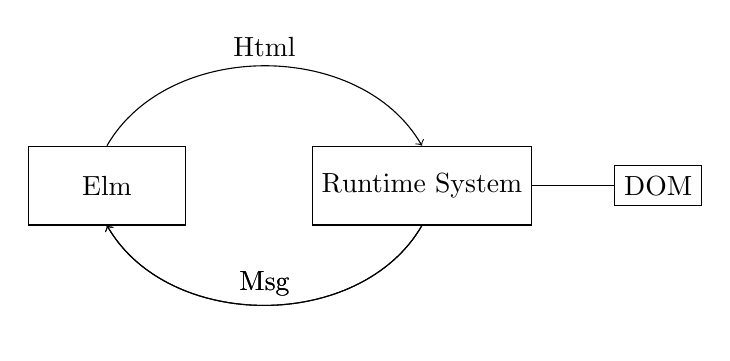
\begin{tikzpicture}
  % Nodes
  \node (p) [rectangle, draw, minimum height=1cm, minimum width=2cm] at (0, 0) {Elm};
  \node (i) [rectangle, draw, minimum height=1cm, minimum width=2cm] at (4, 0) {Runtime System};
  \node (d) [rectangle, draw, minimum height=0.5cm, minimum width=1cm] at (7, 0) {DOM};
  % Arrow
  \draw[->] (p.north) to[out=60, in=120] node[midway, above] {Html} (i.north);
  \draw[->] (i.south) to[out=-120, in=-60] node[midway, above] {Msg} (p.south);
  \draw[->] (i.south) to[out=-120, in=-60] node[midway, above] {Msg} (p.south);
  \draw[] (i) -- (d) node[midway, above] {};
  % Header
\end{tikzpicture}

  \caption{Elm Architecture (Figure adapted from \cite{elmFig})}
  \label{fig:elmArchitecture}
\end{figure}

\subsection{Module Architecture}

In this application, the Elm-box is a module, while the runtime system, is the
core itself. The core invokes all modules, all of which, should have these three
functions, \lstinline{init}, \lstinline{update}, and \lstinline{view}.

\paragraph{Init} Returns a collection of key-value-pairs, which represent
the state of the core.

\paragraph{Update} Returns a collection of key-value-pairs, which
overwrite existing key-value-pairs in the state, or are appended to the state.
Invoked every time a \textit{Msg} is sent.

\paragraph{View} Returns a collection which represents \gls{html},
which is rendered by the core.

A module is initialized by invoking the \textbf{init} method, which returns a
state. This can be seen in figure \ref{fig:moduleInit}. After the state
initialization, the modules' \textbf{view} method is invoked, which initializes
the \gls{ui} for the user, which can be seen in figure \ref{fig:moduleInitView}.

\begin{figure}
  \centering
  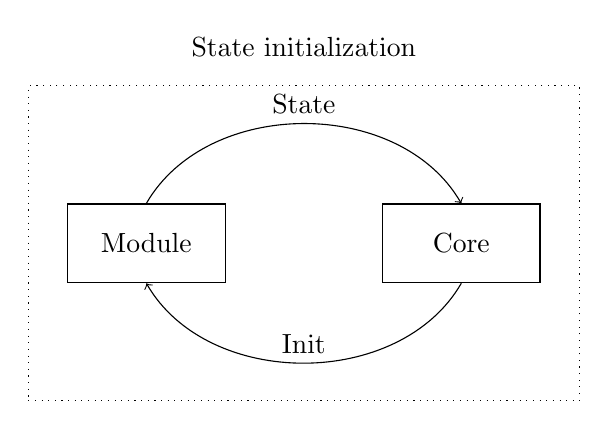
\begin{tikzpicture}
  \node [rectangle, draw, minimum height=4cm, minimum width=7cm, dotted] at (2, 0) {};
  \node [] at (2, 2.5) {State initialization};

  \node (i) [rectangle, draw, minimum height=1cm, minimum width=2cm] at (4, 0) {Core};
  \node (p) [rectangle, draw, minimum height=1cm, minimum width=2cm] at (0, 0) {Module};
  \draw[->] (p.north) to[out=60, in=120] node[midway, above] {State} (i.north);
  \draw[->] (i.south) to[out=-120, in=-60] node[midway, above] {Init} (p.south);
\end{tikzpicture}

  \caption{Module state initialization stage}
  \label{fig:moduleInit}
\end{figure}

\begin{figure}
  \centering
  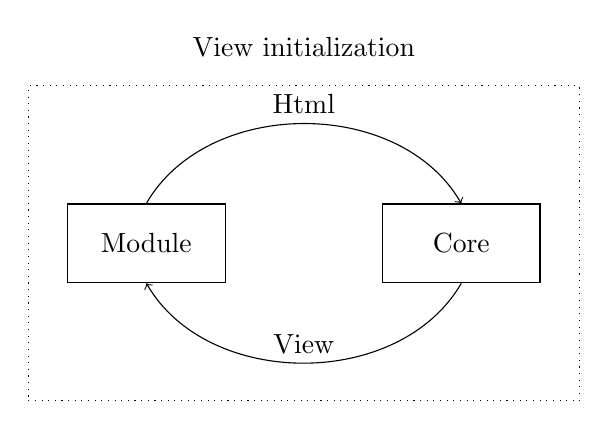
\begin{tikzpicture}
  \node [rectangle, draw, minimum height=4cm, minimum width=7cm, dotted] at (2, 0) {};
  \node [] at (2, 2.5) {View initialization};

  \node (i) [rectangle, draw, minimum height=1cm, minimum width=2cm] at (4, 0) {Core};
  \node (p) [rectangle, draw, minimum height=1cm, minimum width=2cm] at (0, 0) {Module};
  \draw[->] (p.north) to[out=60, in=120] node[midway, above] {Html} (i.north);
  \draw[->] (i.south) to[out=-120, in=-60] node[midway, above] {View} (p.south);
\end{tikzpicture}

  \caption{Module view initialization stage}
  \label{fig:moduleInitView}
\end{figure}

Since the \gls{ide} is written in both TypeScript and Rust, a method of encoding
type information when crossing between the TypeScript and Rust environment was
needed. It was achieved by simply typing \gls{json} objects, so while the state
could be represented as any \gls{json} object, it was instead represented as
nested \gls{json} objects, where, all values, except \textbf{null}, where
encoded as an object with one field, being the type of the object, and then the
value. So an int would be \textbf{\{ int: 0 \}}.

The reason for representing a JSON object as key-value pairs, is that this could
be easily translated to a Rust representation of the same type, using the
\textit{Serde} crate. This allows for creating Rust structs which represents
JSON objects, and creates an automatic encoder/decoder between Rust and
\gls{json}. Using the \textit{ts\_rs}, we could also automatically create the
TypeScript type that represents the automatically encoded/decoded \gls{json}.
This ensures a good cooperation between the \textit{frontend} and
\textit{backend}.

\subsection{IDE lifecycle}

The general idea was that for each possible \gls{dom}-event, there would exist a
way to send a Msg. Each Msg contains a Msg name, and some value, which enabled
pattern matching on Msg, similar to Elm, for modules, so each module could
choose to act on a Msg or not. So, after the initialization of the \gls{ide},
any time the user interacted with the \gls{gui} the modules would react to the
Msg. The trivial plugin, would simply return an empty state on \textbf{init} and
\textbf{update}, while on \textbf{view}, it would return a \textit{frag}
element, which is a React element that evaluates to no \gls{dom} change.

In listing \ref{lst:pluginCounterExample}, an example of a counter module can be
seen. This module initializes a state, containing the field \textbf{"counter"},
with the value \textbf{VInt 0}.

The \textit{update} function the module exposes, matches on a \textbf{"counter"}
msg, with a \textbf{VInt i} value. If the given Msg matches this, then the
module adds to the \textbf{"counter"}-field, the value from the Msg, which is
$1$.

Finally, the \textit{view} function renders a button, which when pushed by a
user, sends the \textit{counter-Msg}.

\begin{center}
  \lstinputlisting
    [ language=Haskell
    , caption={Counter Module (Haskell)}
    , label=lst:pluginCounterExample]{./code/plugin-counter-example.hs}
\end{center}

\subsubsection{Module purity}

One important thing in this architecture, is the pureness of module. The state
of a module needs to be kept in the core application, and not in the module
itself. The reason for this is twofold. It allows for the possibility of the
core to be optimized in the future, as modules which do not react to a certain
msg-state combination, can be noticed, and ensure modules are not unnecessarily
invoked. It also lowers the complexity for module developers, as it is easier to
reason about modules if \textit{all} they do is read or write to some state.

If we have the modules $A$ and $B$, where their relationship is $A \to B$,
meaning $A$ \textit{invokes} $B$ by sending some Msg, which $B$ reacts too, and
we want something to happen before $B$ reacts, we can add a new module, $C$,
which also reacts to the same Msg, but if we know the name of the module $B$,
we can set the name of module $C$ to be \textit{above} the order, relative to
$B$, ensuring that $C$ always triggers before $B$.

\subsection{Module v2 Cons}

\paragraph{Not modular} This setup is also not really modular, as a single
module cannot invoke another module without being impure. The only way to
invoke/trigger another module, is to throw a \textit{Msg}, which would trigger
an update -> view -> cycle. So a module cannot \textit{listen} for a single
message, all modules are triggered by the same \textit{Msg}, and handled
accordingly, synchronously.

\paragraph{Synchronous Module Invocation} If a Msg triggers a computational
heavy method, the \gls{ide} will \textit{hang}, and act \textit{sluggish} until
the computation has finished. This would also affect \textit{all} modules,
since they are invoked in order, regardless of if they actually change the
state or view.

\paragraph{Ever-growing State} There was no way to remove a field on the state,
the state is appending/overwriting -only, which was a side effect of the
\textit{solution} to state collisions.

\subsubsection{State Collision} \label{sec:collision}

A state collision occurs when two or more modules updates the same field, during
the same update-cycle. This issue also occurs when folding two states. After any
update-cycle, we were left with a list of states, which needed to be coalesced
into a singular one. There are several different ways to correct a collision
between two states:

\begin{enumerate}
  \item If the states are of same type:
    \begin{enumerate}
      \item If the value from one of the colliders are unchanged from the previous state:
        \begin{enumerate}
          \item Keep the new value OR Keep the old value
        \end{enumerate}
      \item Else
        \begin{enumerate}
          \item Apply the types' semigroup operator to the fields.
        \end{enumerate}
    \end{enumerate}
  \item Else
    \begin{enumerate}
      \item If the value from one of the colliders are unchanged from the previous state:
        \begin{enumerate}
          \item Keep the new value OR Keep the old value
        \end{enumerate}
      \item Else
        \begin{enumerate}
          \item Keep the left-hand side value OR Keep the right-hand side value
        \end{enumerate}
    \end{enumerate}
\end{enumerate}

Since the states are ordered by the name of the module they come from, we
have a consistent ordering of left-hand side and right-hand side. Due to the
fact that module invocation is synchronous, and ordered. If the same modules
gives a collision on the same input, (given that all modules are pure), the
resulting state will be the same every time. The problem is that applying some
function on the values could be an unwanted way to resolve collisions. The
standard way will be to log the collision, and then drop both states. Even
if two states have $A$ and $B$ amount of fields, and just one collision, we will
drop $A + B$ amount of fields.

This problem of resolving state collision only occurs because each module
returns a subtree of the state. We then have to analyze the new coalesced tree
for each new subtree that is added, to figure out if there occurs any collision.
And then notifying the module developer of which field this collision occurred
on, and which modules tried to modify that field.

\section{Module V.3} \label{sec:mod3}

The third and hopefully final, plan:

\begin{enumerate}
  \item Everything is a module
  \item Modules can \textit{invoke} modules
\end{enumerate}

A module only exposes two functions:

\paragraph{Init} Returns nothing

\paragraph{Handler} Returns nothing

In the previous architecture version, each module directly changed the state,
which caused issues. Instead, each modification a module does, \textit{acts}, as
a direct modification, but is in fact, translated to a DSL which can be analyzed
for possible collisions. This was discovered to be a need, as in the new
version, the \gls{ui} was also restructured, to allow for less re-rendering, and
this restructuring, made it clear that changing the state, or changing the
\gls{ui} is just tree manipulations, which will be discussed more later.

\subsection{Zero core architecture and microservice architecture}

The new plan came with a change of viewpoint. Think of
\textit{everything being a module}, this pushed for a modularization between the
then tightly coupled parts, the \textit{frontend} and \textit{backend}. As
mentioned, having two different languages could allow for easier support of
modules written in different programming languages, but for this to work in an
optimal way, both the \textit{frontend} and \textit{backend} should be loosely
coupled. This is an equivalent architecture to microservices.
\todo{Add diagrams and examples}

\subsection{Vanilla TypeScript}

Instead of using React as the frontend framework, TypeScript was chosen, which
simplified the integration between the backend and frontend, as the complexity
of React's state management could be avoided, along with React's hydration.
Given the rendering was now more \textit{hands-on}, the core could expose a lot
of the functionality for rendering, which modules could change. This would
increase the difference between the \gls{jsms} and \gls{rsms}, as the backend
was not privy to this API, but this was not seen as an issue, as this API would
turn module non-pure.

\subsubsection{Removing abstractions}

It became prudent, due to the change of architecture, to change the entire
frontend, moving away from React, and using \textit{bare-bones} TypeScript. This
would enable easier integration into the \gls{jsms}.

\subsection{Core Modifications}

Learning from the issues outlined in section \ref{sec:collision}, instead of a
module returning the new core, it will rather return a set of instruction on
\textit{how} the core is to be modified, resulting in what the module developer
wants the core to be. The reason for turning it around in this manner, is that,
the new architectural change also came with a change on how the \gls{ui} is
modeled, as it is now up to the core to figure out an inexpensive way to do
rendering. Since the core has \gls{ui}-structure which is a representation of
what the \gls{dom} should be, it can be treated as a Virtual-\gls{dom}, similar
as to how React does it. This also means that there could be a collision on
\gls{ui}-change, as well as on a state-change. Instead of solving the equivalent
problems twice, it was decided to try to treat the issues with collisions in
state and \gls{ui} as the same issue; its some form of tree-manipulation. We
could then reduce the amount of needed methods on the module instance, to two.
One for initializing the state, and one for handling events. In \ref{lst:cm},
we have a \textbf{CoreModification} type, which has two fields, one for the
state, and one for the \gls{ui}.

\begin{center}
  \lstinputlisting
    [ language=Rust
    , caption={Core Modifications (Rust)}
    , label=lst:cm
    , firstline=12
    ]{./core/src-tauri/core-std-lib/src/core_modification/mod.rs}
\end{center}

\subsection{Tree Manipulation}

This restructure changes the way the view is rendered. Instead of the view being
re-rendered for each state-update, the view, or \gls{ui}-hierarchy, is only
modified by modules. This modification is similar to the earlier state
modification, so a unified algorithm to solve this can be used. If there is an
easy way to translate a \gls{ui} modification to a state modification, and back
again. To solve this, instead of having a module return the actual
modifications, meaning, the updated core, a module returns a set of instructions
of what to do with the core.

\begin{center}
  \lstinputlisting
   [ language=Rust
   , caption={Instruction (Rust)}
   , label=lst:inst
   , firstline=6
   , lastline=16
   ]{./core/src-tauri/core-std-lib/src/instruction/inst.rs}
\end{center}

In the listing \ref{lst:inst}, it is clear how the \textbf{Instruction}-set makes the
modification of the core, a kind of group, as given by the definition
\ref{def:group}. Intuitively, for any \textbf{Instruction}, there exists
an \textit{inverse} one, such that the definition \ref{def:inv} is upheld. If we
add some value to the state, we can find an remove instruction that removes
that field from the state, as shown in listing \ref{lst:inst}, in the
\textbf{combine} method.

\begin{remark}
  The \textbf{combine} method does not recursively check the \textbf{Then}
  instruction for \textbf{Instruction}s that lead to a \textbf{NoOp}, but in the
  core \gls{ide}, there is an optimization step that does this.
\end{remark}

To formalize this, that the \textbf{Instruction}-set is an group, we can look at
a subset, since \textbf{Instruction} is parameterized by some type \textbf{T},
we will look at it when \textbf{T} is \textbf{Value}, noted by the subscript
\textbf{val}.

\begin{theorem}[Instruction Group] \label{thm:intr}
  Let $\Sigma$ be the set of all strings, $Val$ be the set of all
  \textbf{Values}, $Html$ be the set of all \textbf{Html} variants, and
  $Inst_{val}$ be the set of all \textbf{Instruction} defined as:
  $$
    NoOp = \left \{ noOp \right \}
  $$
  $$
    NoOp \in Inst_{val}
  $$
  $$
    Add_{val} = \left \{ (x, y, z) \vert x \in \Sigma, y \in \Sigma, z \in Val \right \}
  $$
  $$
    Add_{val} \in Inst_{val}
  $$
  $$
    Rem_{val} = \left \{ (x, y, z) \vert x \in \Sigma, y \in \Sigma, z \in Val \right \}
  $$
  $$
    Rem_{val} \in Inst_{val}
  $$
  $$
    Then_{val} = \left \{ (x, y) \vert x, y \in Inst_{val} \right \}
  $$
  $$
    Then_{val} \in Inst_{val}
  $$
  For any $x \in Add_{val}$ there exist a unique $y \in Rem_{val}$, such that:
  $$
    x \oplus y = noOp
  $$
\end{theorem}

The theorem \ref{thm:intr}, unfortunately, cannot be encoded in Rusts type
system, but when implementing $combine$, we can map the variants along with the
specific fields being added ($Add$), modified ($Mod$), or removed ($Rem$), to get
a more optimized instruction set. If we are modifying a value on field $foobar$,
but in the same instruction set, remove it, then the modifying instruction is an
$NoOp$. This optimization can be found in appendix \ref{app:a}.

Like writing direct binary to develop a program, writing \textbf{instruction}s to
change the core is quite abstract for most developers so to facilitate development
of modules, a helper class was created, which \textit{translates} modifications
to instructions. As shown in listing \ref{lst:ui-builder} and
\ref{lst:state-builder}, a module developer simply invokes different methods on
the builder, eventually building a \textbf{CoreModification}, to be sent.

\begin{center}
  \lstinputlisting
   [ language=Rust
   , caption={
     UI Builder (Rust) showcasing how to add an empty \gls{html} div element to
     the root \gls{html} element.
   }
   , label=lst:ui-builder
   ]{./code/module-ui-builder.rs}
\end{center}

\begin{center}
  \lstinputlisting
   [ language=Rust
   , caption={
     State Builder (Rust) showcasing how to add a \textit{count} field to the
     state, also showcasing how Rust can infer that the i32 type $0$ is
     a \textbf{Value::Int} type.
   }
   , label=lst:state-builder
   ]{./code/module-state-builder.rs}
\end{center}

This allows for an ergonomic way for module developer to create modifications on
the core, without having to understand the syntax of the
\textbf{Instruction}-set.

\subsection{Backend Agnostic Frontend}

Since we are using the framework Tauri to implement the \gls{ide}, the \gls{ide}
is split to two, loosely coupled parts. The \textit{frontend} and
\textit{backend}. The frontend acts as a thin wrapper around the core \gls{api},
enabling different \textit{runtimes} to handle module management, while the
frontend waits for events, and renders the \gls{gui}. This structure allows for
future maintainers of the \gls{ide} to be able to \textit{trivially} switch
runtime, if they wanted to use some other language to implement the runtime
system in, like PureScript, Gleam or Haskell, all of which can target
JavaScript, then they could.

\subsection{Making the Core evaluate modifications asynchronously}

Due to Rust first class focus on concurrency, it was trivial to make the core
modifications run asynchronously. In previous iterations, the core evaluated
one event at a time, waiting until all modules had finished their computations,
before emulating the change and allowing for the next event to be evaluated. But
this caused a noticeable \textit{lag} if an event was long. This was solved by
changing the core modification evaluation from a simple method to be invoked, to
an \gls{mpsc} channel system. Using \textit{tokio}, a Rust crate for
asynchronous development, a channel for core modifications was created, and
instead of the core collecting all modifications, each module is invoked and
\textit{awaited} for in a separate thread, where in each module, if they have a
core modification, sends the modification to the core channel, which works on
a first come, first server basis. Here the core can evaluate the changes, also
on a separate thread.

\section{Testing} \label{sec:testing}

A zero-core \gls{ide} is equivalent to a microservice architecture, in that
testing is important to ensure changes in one module does not inadvertently
affect another. This is commonly achieved by using \textit{pipelines}, a part
of the \gls{cicd} process, where we run several \textit{jobs} whenever we make a
change to our application. If we are bundling different modules together, and
serving that as an \gls{ide}, we want to ensure that a change to a module does
not negatively affect the other. This is where \textit{pipeline jobs} come in,
as each \textit{job} test some part of our \gls{ide}. While it is cheaper to
\textit{spin} up an instance of the \gls{ide} in a pipeline, than an application
dedicated to serve millions of users, we still want to avoid doing this
unnecessarily. This is why we split up our testing into different stages.

\subsection{Mocking}

Due to the \textit{pureness} of modules, mocking can be achieved easily, and
therefore, modules can be tested alone, which is good, because testing a
singular module is inexpensive. There are several ways to do this mocking in our
architectural setup. For both the \gls{jsms} and \gls{rsms}, there are
\textit{mock-cores}, which can mock the expected functionality of the Core
instance, which we can extend to evaluate actual modifications, ensuring we can
assert that some state or \gls{ui} change has occurred after an Event has been
sent.

\subsection{Unit Testing}

A module developer should create unit tests for their module. This can easily be
done, and tested many times, due to the light-weightiness of a module. This,
together with mocking, ensures we can test our modules, as if they were in a
\gls{ide}. Which means we can ensure changes made to a module is non-breaking.

This also applies to maintainers of the \gls{ide}, as maintaining the core
functionality and \gls{api} of our library, means documenting possible breaking
changes, which unit tests can help ensure.

\subsubsection{UI Testing}

We can also combine this with existing testing libraries, like \textit{Playwright}\footnote{\url{https://playwright.dev/}},
which can enable us to create tests specifically for UI behavior. In the case of
\textit{Playwright}, our \gls{ui} testing is dependent on that our
\textit{mock-core} has the necessary functionality to transform the
\textbf{Html} type we have implemented, to actual \gls{html}, which can be
rendered on a webpage, or \textit{headless}, in \textit{Playwright}s case, so
that \textit{Playwright} can assert the state of our \gls{dom}.

\subsection{Module Family Testing}

If a module changes some feature, let's say in the editor functionality, the
module family tree encompassing this functionality needs to be tested, to ensure
nothing breaks. This means creating tests that use all the modules in a family,
and asserting that the state and \gls{ui} behave as expected. In the case of
the editor functionality, that after the Event \textit{open-file} is sent with
a path to some file, that there exists a \textit{textarea}-\gls{html}-element in
the \gls{dom}, with the same contents as the file.

\subsubsection{Contract Testing}

As a module developer, on is designing some kind of \gls{api}, but the developer
has no say in how a consumer of the \gls{api} consumes it. In a microservice
architecture, the common way to work around this, is to version control the
\gls{api} by prefixing \textit{v*} in front of all endpoints in the \gls{api},
where star, (*), is the version of the \gls{api}. This way, the \gls{api}
designer can develop new \gls{api}s, without worrying about breaking
functionality that consumers of the \gls{api} depend on. This, however, usually
means having to maintain equivalent \gls{api}s in parallel, until one decides
to deprecate an older less used version, forcing consumers to move on to the
newer version of the \gls{api}.

Instead of relying on such a versioning system, module developers could use
\textit{contract testing}.

\paragraph{Contract Testing} Imagine some \gls{api}, and several consumers,
$A, B, C$, The \gls{api} developer is serving some data, in this case an
integer number, which all the consumers use. One day, the developer finds out
that using integers is not optimal, and want to move on to using floating point
numbers instead. Changing the \gls{api} outright could bring issues, as the
consumers might rely on the \gls{api} being an integer, instead of a float. But
the change is needed, or wanted, at least. In this scenario, it is \textit{easy}
to inform all the consumers of the \gls{api}, but if the consumer count
increases tenfold, this is more difficult. A notice can still be sent, but it is
not feasible to ensure all consumers commit time to change their ways. Contract
testing ensures that, if a change like this occurs, the maintainer of the
\gls{api} is notified by which consumer this change breaks.

The issue is to create these contracts. Using frameworks like Pact \cite{pact},
a developer creates a \gls{dsl} test, where they describe how the provider or
consumer reacts to certain interactions. But since everything is a module, we
can automate this.

\subsection{Automating Contract Testing}

This process could be partially automated, as all modules have to register the
event they want to handle. Furthermore, all events thrown are also explicitly
done through the core instance, meaning a \textit{test-core} could be created,
which registers which event is thrown from what module, and all dependencies
between modules can be noted.

\subsection{End-To-End-Testing}

The final step in the testing pipeline, is to test the entire application
together. This is known as \gls{e2e}. \gls{e2e} is expensive, compared to the
other steps, as we have to load the entire application in the pipeline, and test
all interactions. This, of course, is the easiet way to cover all edge-cases, but
since it is the whole application being tested, harder to figure out what caused
a failure. Our \gls{ide} can be saturated with events in the \gls{e2e} step of a
pipeline, as all user interactions are translated into events, this ensures a
module developer can narrow down what modules are at fault, by what modules
\textit{subscribe} to that event.

\section{Module Developer Tools}

The module developer experience is an important aspect of a zero-core
architecture. A good way to improve this experience, is by providing good
tooling.

\subsection{Module Dependency Visualization}

\todo{Still being developed}

\subsection{Module Isolation Testing}

\todo{Still being developed}

This is as simple as creating a minified version of our \gls{ide}, that has
extra tools for mocking Events.

\subsection{Module Boilerplate Generation}

\todo{Still being developed}

This \gls{cli}-tool enables a developer to quickly get started on developing
modules, as the tidous work of setting up a project can be automated away.

\section{Modules}

\paragraph{Event Type} In listing \ref{lst:moduleEvent}, one can see the
structure of an event type. This allows for modules to pattern match on specific
events, and unlike, as in the previous version, modules can \textit{subscribe}
to specific events to react to. This changes the structure of the module
architecture to go from one wherein the core is a terminal object, to a more
\textit{complicated} one, in which module families can form.

\begin{center}
  \lstinputlisting
    [ language=Rust
    , caption={Module Event (Rust)}
    , label=lst:moduleEvent
    , firstline=14
    , lastline=41
    ]{./core/src-tauri/core-std-lib/src/event/mod.rs}
\end{center}

This forms our \textit{request} and \textit{response} type, making the
equivalence with a \gls{rest} \gls{api} obvious. The clients and consumers
of the \gls{api}, are the modules which can be seen in listing \ref{lst:mod}.

\begin{center}
  \lstinputlisting
    [ language=Rust
    , caption={Module trait (Rust)}
    , label=lst:mod
    , firstline=12
    , lastline=16
    ]{./core/src-tauri/core-module-lib/src/lib.rs}
\end{center}

A module can interact with the core, by getting the state, \gls{ui},
\textit{throwing} an event, registration themselves to \textit{handle} an
event, or to \textit{send} a \textbf{CoreModification}. In listing
\ref{lst:core}, we can see this core trait.

\begin{center}
  \lstinputlisting
    [ language=Rust
    , caption={Core trait (Rust)}
    , label=lst:core
    , firstline=6
    , lastline=18
    ]{./core/src-tauri/core-std-lib/src/core.rs}
\end{center}

Since a module updates the core by \textit{choosing} to send a
\textbf{CoreModification}, through a \gls{mpsc}-channel, a module can run an
expensive computation on another thread, while \textit{ending} their
invocation, ensuring a smooth \gls{ide} experience.

Here are some examples of modules implemented using the proposed architecture.


\subsection{Module Tools}

When developing against a module architecture, having tools to help debug issues
is useful. \dots

Some examples of issues we have experienced when developing modules are as
follows:

\begin{enumerate}
  \item Incorrect handler registration
  \item Incorrect Event name
  \item Incorrect arguments in response
  \item Incorrect arguments in request
  \item Incorrect State
  \item Concurrent Events
\end{enumerate}

Most of these issues relate to the Event system, so being able to mock events
is a useful tool. Luckily, this is quite simple to implement. In
picture \ref{pic:eventMock} we can see this in action.

\begin{figure}[H]
  \centering
  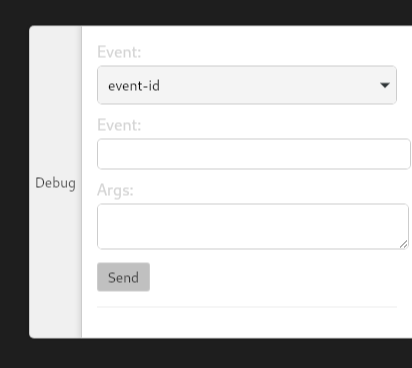
\includegraphics[width=0.75\textwidth]{event-mocking.png}
  \caption{
    Event Mocking module that adds a simple pop-up menu for manually sending
    Events, with specific arguments
  }
  \label{pic:eventMock}
\end{figure}

When mocking in \gls{rest}-\gls{api} development, one creates the expected
response, which is usually a \gls{json}-file. The same is done here, where the
\textit{Args} field in this form expects the argument to be in \gls{json}. This
is helpful, as other testing libraries, like \textit{Playwright} does the same,
and the \gls{ide} logs the Event arguments in the same formatting, meaning we
can simply copy-paste the Event argument we want to mock, into the field.

In the picture \ref{pic:debugState}, we can see a module which helps visualize
the current state of the \gls{ide}, in a tree-graph.

\begin{figure}[H]
  \centering
  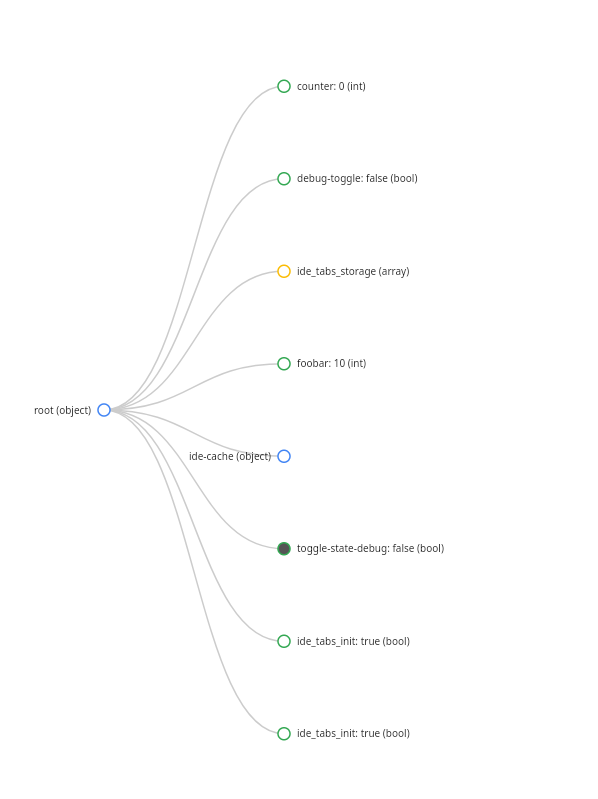
\includegraphics[width=0.75\textwidth]{debug-state.png}
  \caption{
    Debug-tool for visualizing the current \gls{ide}-state
  }
  \label{pic:debugState}
\end{figure}

\subsection{Magnolia Dependency Graph Visualizer}

In Magnolia, as in many other languages, one cannot have a cyclic dependency.
This means that the dependency graph of a Magnolia project should be a
\gls{dag}. And since Magnolia has such a focus on reuse, the dependency graphs
in a Magnolia project could be quite large. Which means the cycles could be
quite long, which would make resolving the cyclic dependency issue complicated.
One way to help a developer, would be to give them a tool to visualize the
dependency graph, so that they could see what modules are connected. Using the
Magnolia library as the input, we can create a visualization of the dependencies
in Magnolia. Using two modules, one for \textit{parsing} the Magnolia library,
finding all packages, and their dependencies, and another for visualizing
this.

\begin{center}
  \lstinputlisting
    [ language=Rust
    , caption={
      Magnolia library parser Module \textit{subscribing} to an
      \textit{get\_magnolia\_graph } Event (Rust)
    }
    , label=lst:magnoliaLibParserSub
    , firstline=33
    , lastline=36
    ]{./modules/magnolia\_dependency/src/lib.rs}
\end{center}

In listing \ref{lst:magnoliaLibParserSub}, the module is invoking the
\textit{add\_handler} method on an object that implements the \textit{Core} trait,
(\ref{lst:core}), and passing \textit{get\_magnolia\_graph} and
\textit{MODULE\_NAME}. This means that Events with the event name
\textit{get\_magnolia\_graph}, will trigger this module. It's \textit{this}
module, because we have to pass the name of the module handling the event.

We can therefore invoke this Module by simply triggering the subscribed Event.

Due to Rust's type safety, there is a lot of \textit{noise}, especially because
we are working with recursive data structures, with optional values. In listing
\ref{lst:magLibParserSimple}, we can see a simplified version of the module
handler, but this is not valid Rust code, the full code for the module can be
found in appendix \ref{apx:b}.

\begin{code}[H]
  \lstinputlisting
    [ language=Rust
    , caption={Simplified magnolia library parser Module (Rust)}
    , label=lst:magLibParserSimple
    , numbers=left
    , numberstyle=\tiny\color{gray}
    ]{./code/mag\_lib\_simple.rs}
\end{code}

The above code (\ref{lst:magLibParserSimple}), we are handling Events with the name
\textit{get\_magnolia\_graph}, (line 3), and getting the path that is supplied in
the Event argument, (line 4). In line 4 we then create a \textit{key}, which we
use to check if this graph has been created yet, by checking the state (line 6).
If this graph does exist, we \textit{respond} by throwing an Event with the
existing graph (line 7 to 9). If it does not exist, we create it by calling the
\textit{get\_graph} function, (left out for brevity), which recursively finds
files in the supplied path, using RegEx to find the packages, and their
dependencies. We then end by \textit{responding} with the created graph,
(line 12), and store it in the state, with the key (line 13 to 16). The
resulting response can be seen in listing \ref{lst:magLibParserRes}

\begin{code}[H]
  \begin{lstlisting}[language = TypeScript, label=lst:magLibParserRes, caption={Magnolia library parser response (TypeScript)}]
    {
      event: {
        event: "graph",
        args: {
          list: [
            {
              obj {
                name: { str: string },
                dependencies: { list: [{ str: string }] }
              }
            }
          ]
        }
      }
    }
  \end{lstlisting}
\end{code}

The module responsible for rendering the graph, uses
\textit{d3}\footnote{\url{https://d3js.org/}}, a visualization library for
JavaScript. \textit{d3} expects \textit{nodes} and \textit{links}, specified in
listing \ref{lst:d3Type}.

\begin{lstlisting}[language = TypeScript, label=lst:d3Type]
  type Node = { id: string, name: string };
  type Link = { source: string, target: string };
\end{lstlisting}

But due to how types are encoded in our Value type, as seen in
\ref{lst:magLibParserRes}, some translation is necessary. We have to go from the
type \textit{Value}, to
\textit{
  list of objects, with two fields, name and dependencies, of type string and
  list of string, respectively}
This translation can be seen in \ref{lst:depVisMod}. Left out, are the steps
verifying that the event has an argument, (since its optional to pass one), and
that the argument is of the list variant of \textit{Value}. The full source code
can be found in appendix \ref{apx:b}. Since the list variant can contain any
\textit{Value} variant, we filter the list by whether it is an object variant,
(line 2), we then transform each element in the list, into a intersection of the
types \textit{d3} expects, (\ref{lst:d3Type}). The questionmark syntax on line
4, where we declare the \textit{id} variable, means that if any of the
expressions on the left are undefined, the resulting expression is undefined.
Since the object variant of \textit{Value} does not necessarily contain the
\textit{name} field, or is of the kind \textit{str}. On line 9 to 13, we are
getting all the dependencies from the object, with a helper method,
\textit{tObjLookUpOr}. This method does a \textit{lookup} on the supplied field
on an object, and a typecheck. If the object does not exist, or is not of the
correct type, the passed fallback value is returned instead, in this case, an
empty list (line 10). Since we know the value is an list, we can safely access
it, (line 11), and filter by the string variant, and transforming the
\textit{Value} to a string primitive, (line 11 to 13).

\begin{code}[H]
  \lstinputlisting
    [ language=TypeScript
    , caption={Dependency visualiser module (TypeScript)}
    , label=lst:depVisMod
    , numbers=left
    , numberstyle=\tiny\color{gray}
    , firstline=160
    , lastline=174
    ]{./modules/dependency-viewer/module.ts}
\end{code}

In the picture \ref{pic:magLib}, we can see the finished rendering of the
dependency graph of the Magnolia basic library. As mentioned earlier, Magnolia
has a lot of re-use, and therefore dependencies. That makes this visualization
quite \textit{noisy}, as there are a lot of crossing between the dependencies.

\begin{figure}[H]
  \centering
  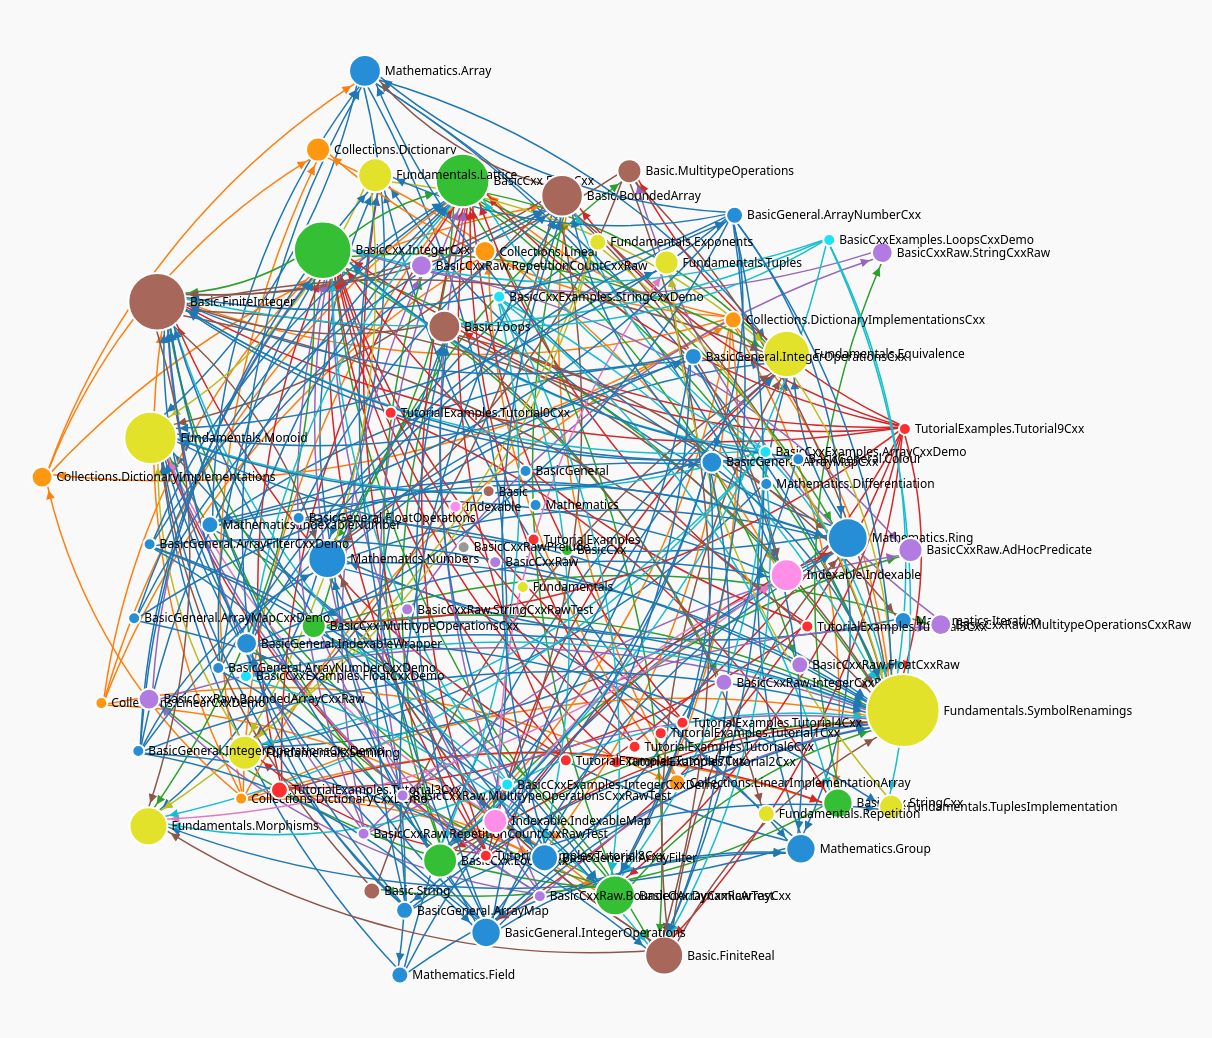
\includegraphics[width=0.75\textwidth]{magnolia-dependencies.png}
  \caption{
    Magnolia basic library dependencies visualized. Each colour represents a
    package, which contains several modules. The size of the nodes vary
    depending on the amount of dependents, (indegree), a module has.
  }
  \label{pic:magLib}
\end{figure}

Luckily, with \textit{d3}, we can mitigate some of the noise. In the picture
\ref{pic:depCont}, we can see the control-panel that our graph module has
created. With the control panel, we can zoom in and out on the graph,
(this can also be done with the mouse), reset our view. This is done with the
help of \textit{d3}, while the final button, find cycles, is implemented by
simply checking the input data for a cycle, and colouring it red with the help
of basic JavaScript and \gls{css}. The remaining sliders are specifically for
the graph ordering itself, where force strength, is with how much force nodes
exert on each other, and link distance is how far a link between two nodes
can/\textit{wants} to be. This, along with the node size scale, scaling how big
a node is depending on how many dependents it has, ensures this visualisation
tool can be used for other programming libraries, not just Magnolia.

\begin{figure}
  \centering
  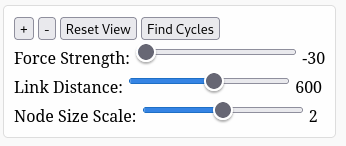
\includegraphics[width=0.45\textwidth]{dependency-viewer-controls.png}
  \caption{
    Control panel, with buttons and sliders for controlling the graph view
  }
  \label{pic:depCont}
\end{figure}

Furthermore, we can highlight the packages we care about, using the filter
panel the module created. In picture \ref{pic:depFil}, all the different
Magnolia packages have been detected, and their corresponding colour has been
added. We can then enable, or disable them.

\begin{figure}
  \centering
  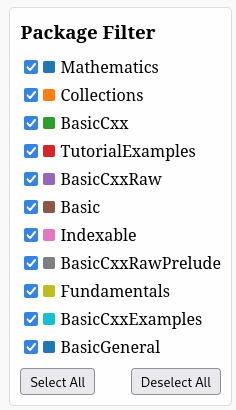
\includegraphics[width=0.45\textwidth]{dependency-viewer-filter.png}
  \caption{List of packages in the graph, that can be toggled}
  \label{pic:depFil}
\end{figure}

In the picture \ref{pic:depDis}, we can see the graph after we have disabled all
other packages, except the \textit{Fundamentals} package.

\begin{figure}
  \centering
  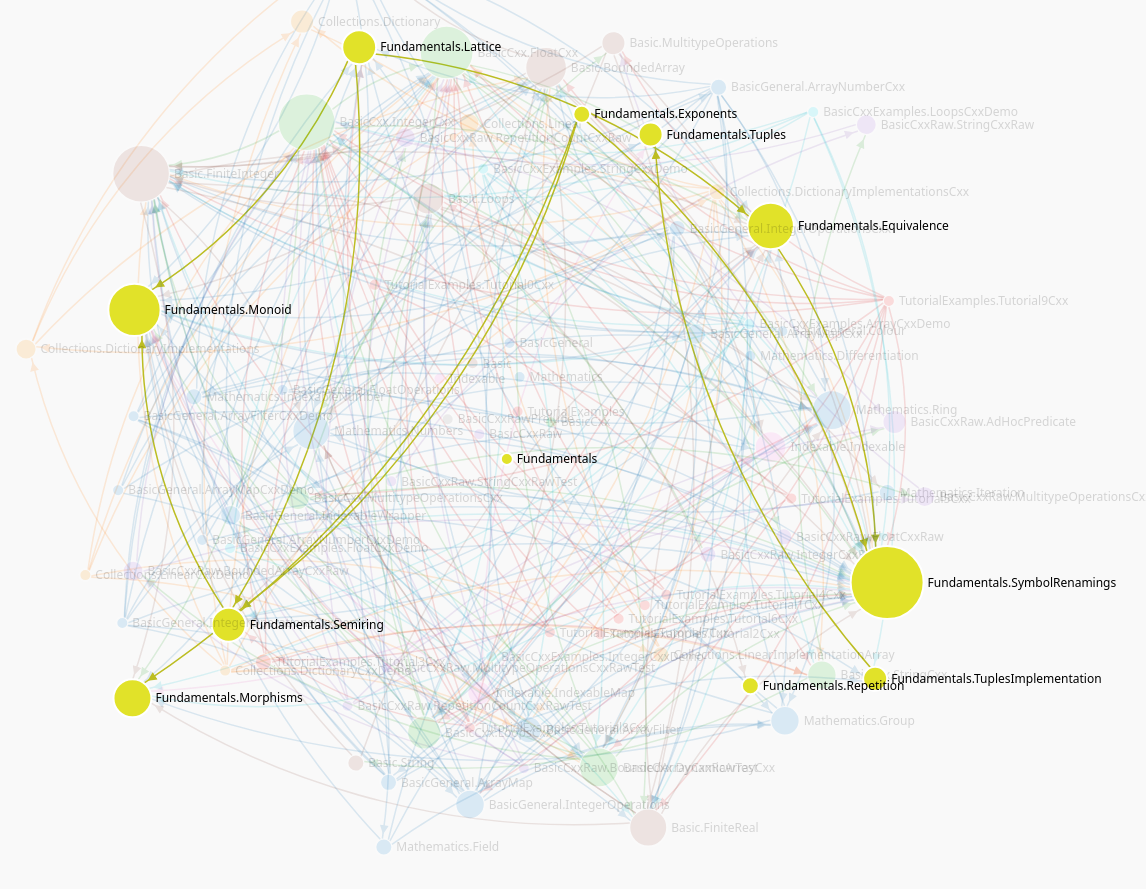
\includegraphics[width=0.75\textwidth]{magnolia-dependencies-filtered.png}
  \caption{
    Magnolia basic library, with just the \textit{Fundamentals} package
    highlighted.
  }
  \label{pic:depDis}
\end{figure}

\subsection{IDE Module Family}

\subsection{Caching}

There are two difficult problems in computer science\footnote{\url{https://martinfowler.com/bliki/TwoHardThings.html}}.
Cache invalidation, naming things and off-by-one errors. Compiler for
programming languages stores compiled code, such that it is not unnecessarily
re-compiled. Similarly, \gls{ide}s like \gls{intellij} or \gls{vscode} store the
application state between sessions, what files where opened, where in the files
one where, etc. In this \gls{ide}, something similar can be done, by using the
\textit{ide\_cache} module. This module declares a field on the state,
\textit{ide-cache}, which everytime the \gls{ide} exits, it writes to a file the
contents of the field, which it reads and adds to the state during the
\textit{PostInit}-event. That way, if existing modules are doing some state
change, they can be trivially refactored to use the cache field instead, by
simply pre-fixing all their paths with \textit{ide-cache}. In the dependency
visualizer, we can prefix the graph storing, with this, and then the generated
graph would be stored across sessions, ensuring a speedier visualisation
process, as we don't have to wait for an, relatively, expensive IO operation.

\subsection{IDE Framework}

An important aspect development, is separation of concerns. This is also
relevant for module development. A module that renders a \gls{dag}, should not
also be responsible for parsing a library and retrievieng the data to be
rendered. The same principle has been applied when developing prototype modules
for this \gls{ide}, the following modules are responsible for the \textit{view}
of the \gls{ide}:

\begin{enumerate}
  \item \textit{ide\_explorer}: Responsible for the file explorer
  \item \textit{ide\_framework}: Responsible for general layout
  \item \textit{ide\_pm}: Responsible for the menu bar
  \item \textit{ide\_tabs}: Responsible for the tabbing system
  \item \textit{ide\_errors}: Responsible in displaying module errors
\end{enumerate}

In the figure \ref{fig:ideLayout}, we have laid out the naming convention we
use when referring to different \textit{places} in the \gls{ide}.

\todo{Create the figure}

The module \textit{ide\_pm}, being responsible for the menu bar at the top of
the \gls{ide}, has an \textit{easy} job, as it just simplifies the creation of
interactive \gls{ui} elements for other modules. With the dependency graph
visualization module, we can create a module which sends the initial Event that
triggers the graph visualization, and have the button be under the \textit{View}
dropdown content.

In picture \ref{pic:ideEx} we can see the ide\_explorer in action, showing the
Magnolia library visualized as a tree-like structure with collapsible folders.
When we click on the \textit{File}, a dropdown appears, where we can click on a
button, \textit{Open Folder}, which sends an Event to \gls{ide}\_fsa, the
module in charge of handling file system operations, where we get in
\textit{response}, all the folders and files in the path we selected. Which we
transform into \gls{html}, and along with some \gls{css}, we get the collapsible
folders.

\begin{figure}
  \centering
  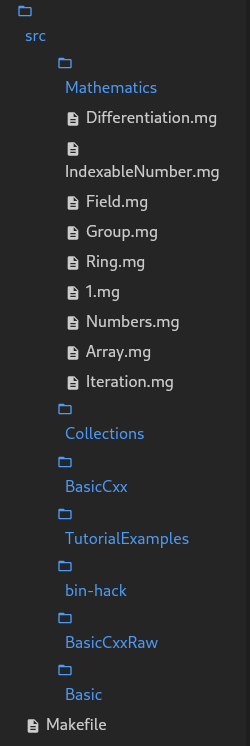
\includegraphics[width=0.25\textwidth]{ide-explorer.png}
  \caption{
    \gls{ide}-explorer module, showing the Magnolia library.
  }
  \label{pic:ideEx}
\end{figure}

There are also some icons, on files and folders, this is done using \gls{css},
in listing \ref{lst:ideEx}, we can see a snippet of this, since we are adding
the file exstension as a class attribute, we can very simply add
style-predicates to our files.

\begin{center}
  \lstinputlisting
    [ language=css
    , caption={
      Module for styling the file explorer, adding an latex icon to all files
      with the \textit{tex} exstension (\gls{css})
    }
    , label=lst:ideEx
    , firstline=152
    , lastline=154
    ]{./modules/ide\_explorer/ide\_explorer\_style.css}
\end{center}

\subsection{Editor Module Family}

The editor module family is coupled with the \gls{ide} framework, as using the
ide\_explorer module, we can open and edit files. By adding a \textit{click}
attribute to the files in the tree, we send an Event to \gls{ide}\_fsa, which
reads the file we clicked on. We know what file we clicked on, because each
\textit{click} attribute has sends an Event with their corresponding path. When
we get the texts contents of the file in response, we create an textarea with
the contents of the file added to it. In picture \ref{pic:editorModule} we can
see this in action.

\begin{figure}
  \centering
  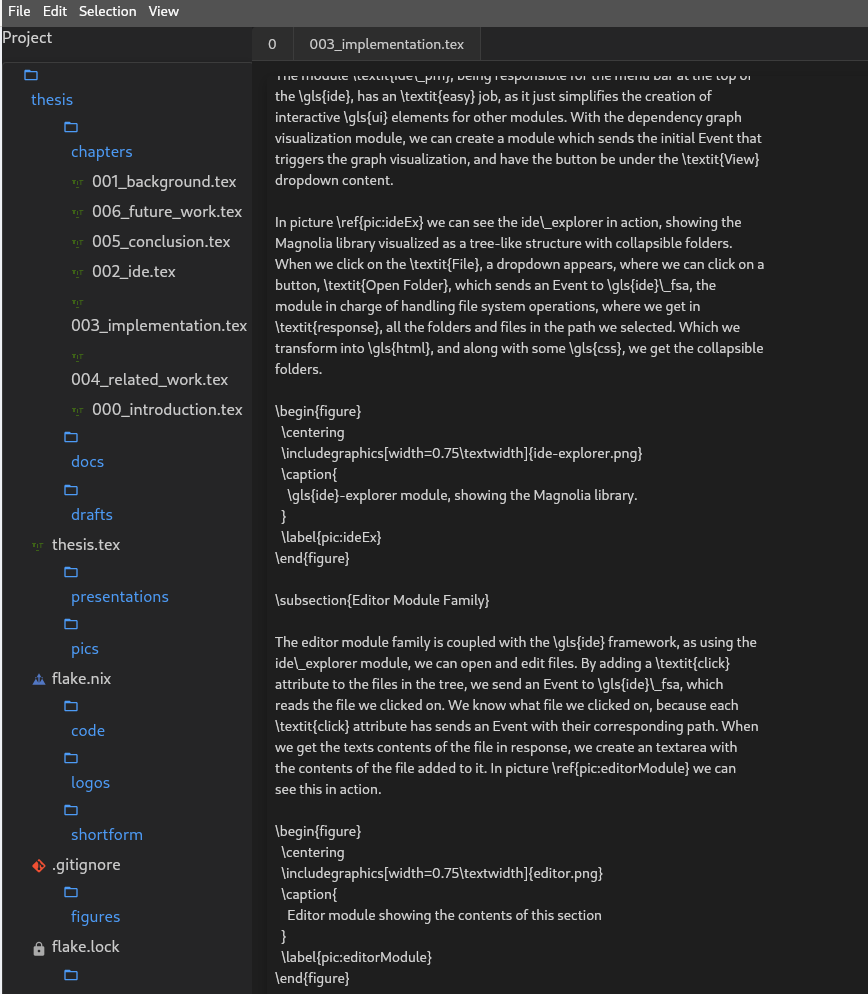
\includegraphics[width=0.5\textwidth]{editor.png}
  \caption{
    Editor module showing the contents of this section
  }
  \label{pic:editorModule}
\end{figure}

\subsection{Magnolia Language Server}

\todo{Implement a rudimentary Magnolia LS}
